\documentclass[10.5pt,compsoc]{CjC}
\usepackage{CJKutf8}
%\usepackage{CJK}
\usepackage{graphicx}
\usepackage{footmisc}
\usepackage{subfigure}
\usepackage{url}
\usepackage{multirow}
\usepackage[noadjust]{cite}
\usepackage{amsmath,amsthm}
\usepackage{amssymb,amsfonts}
\usepackage{booktabs}
\usepackage{color}
\usepackage{cite}
\usepackage{ccaption}
\usepackage{booktabs}
\usepackage{float}
\usepackage{fancyhdr}
\usepackage{caption}
\usepackage{xcolor,stfloats}
\usepackage{comment}
\setcounter{page}{1}
\graphicspath{{figures/}}
\usepackage{cuted}%flushend,
\usepackage{captionhack}
\usepackage{epstopdf}
%\usepackage{ccmap}
%\CJKtilde
%\usepackage{CJKpunct} 
%\usepackage[lite,subscriptcorrection,slantedGreek,nofontinfo]{mtpro2}

%===============================%
% 文章信息
% 作者:-author-cn-
% Author: -author-en-
% 日期: -year-.-month-
% 实验编号: -lab-
% 文章标题:实验 -lab-:-title-cn-
% Title: Lab -lab-: -title-en-
% 使用说明:
% 1. 请直接使用字符逐次全部替换上方的占位符(-xxx-)即可
% 2. 请注意 section 和 subsection 的用法,需要整个块复制使用
% 3. 参考文献使用 BibTeX,需要在同级目录下的 ref.bib 文件中添加参考文献
%===============================%

% 页眉区,分别设置奇数页和偶数页的页眉
\headevenname{
  \mbox{\quad} \hfill  
  \mbox{
    \begin{CJK*}{UTF8}{song}\zihao{-5}
      人\quad 工\quad 智\quad 能\quad 导\quad 论\quad 实\quad 验\quad 报\quad 告
    \end{CJK*}
    \hspace {40mm}
    \mbox{
      \begin{CJK*}{UTF8}{song}
        -year- 年
      \end{CJK*}
    }
  }
}
\headoddname{
  \begin{CJK*}{UTF8}{song}
    -lab- 期 \hfill -author-cn-:-title-cn-
  \end{CJK*}
}

%footnote use of *
\renewcommand{\thefootnote}{\fnsymbol{footnote}}
\setcounter{footnote}{0}
\renewcommand\footnotelayout{\zihao{5-}}

\newtheoremstyle{mystyle}{0pt}{0pt}{\normalfont}{1em}{\bf}{}{1em}{}
\theoremstyle{mystyle}
\renewcommand\figurename{figure~}
\renewcommand{\thesubfigure}{(\alph{subfigure})}
\newcommand{\upcite}[1]{\textsuperscript{\cite{#1}}}
\renewcommand{\labelenumi}{(\arabic{enumi})}
\newcommand{\tabincell}[2]{\begin{tabular}{@{}#1@{}}#2\end{tabular}}
\newcommand{\abc}{\color{white}\vrule width 2pt}
\makeatletter
\renewcommand{\@biblabel}[1]{[#1]\hfill}
\makeatother
\setlength\parindent{2em}
%\renewcommand{\hth}{\begin{CJK*}{UTF8}{hei}}
%\renewcommand{\htss}{\begin{CJK*}{UTF8}{song}}


\begin{document}
\hyphenpenalty=50000
\makeatletter
\newcommand\mysmall{\@setfontsize\mysmall{7}{9.5}}
\newenvironment{tablehere}
  {\def\@captype{table}}

\let\temp\footnote
\renewcommand \footnote[1]{\temp{\zihao{-5}#1}}


\thispagestyle{plain}%
\thispagestyle{empty}%
\pagestyle{CjCheadings}

% 首页特殊页眉
\begin{table*}[!t]
\vspace {-13mm}
\begin{tabular}{p{168mm}}
  \begin{CJK*}{UTF8}{song}\zihao{5-}
    第01卷\quad 第-lab-期
    \hfill
    人\quad 工\quad 智\quad 能\quad 导\quad 论\quad 实\quad 验\quad 报\quad 告
    \hfill
    Vol. 01  No. -lab-
  \end{CJK*}\\
  \begin{CJK*}{UTF8}{song}\zihao{5-}
    -year-年-month-月
    \hfill
    Lab Report of Introduction to Artificial Intelligence
    \hfill
    -month-. -year-
  \end{CJK*}\\
\hline\\[-4.5mm]\hline
\end{tabular}

% 论文标题
\centering
\vspace {11mm}
\begin{CJK}{UTF8}{hei}\zihao{2}
  实验 -lab-:-title-cn-
\end{CJK}
\vskip 5mm

% 论文作者
\begin{CJK*}{UTF8}{fs}\zihao{3}
  -author-cn-$^{1)}$
\end{CJK*}

% 作者单位
\vspace {5mm}
\begin{CJK*}{UTF8}{song}\zihao{6}
  $^{1)}$(南京大学~ 智能科学与技术学院,~ 苏州~ 215100)
\end{CJK*}

% 摘要、关键词、中图分类号、DOI
\vskip 5mm
\centering
\begin{tabular}{p{160mm}}
  \zihao{5-}{
    \setlength{\baselineskip}{16pt}\selectfont{
      \begin{CJK*}{UTF8}{hei}
        摘\quad 要\quad
      \end{CJK*}
      \begin{CJK*}{UTF8}{song}
        中文摘要内容\cite{harris2020array}
      \end{CJK*}
      \par
    }
  }\\[2mm]
  \zihao{5-}{
    \begin{CJK*}{UTF8}{hei}
      关键词
    \end{CJK*}
    \quad 
    \begin{CJK*}{UTF8}{song}
      人工智能导论;实验
    \end{CJK*}
  }\\[2mm]
  \zihao{5-}{
    \begin{CJK*}{UTF8}{hei}
      中图法分类号
    \end{CJK*}
    \begin{CJK*}{UTF8}{song}
      TP
    \end{CJK*}
    \rm{\quad \quad \quad}
    \begin{CJK*}{UTF8}{hei}
      DOI号:
    \end{CJK*}
    \begin{CJK*}{UTF8}{song}
      *投稿时不提供DOI号
    \end{CJK*}
  }
\end{tabular}

% 英文标题
\vskip 7mm
\begin{center}
  \begin{CJK*}{UTF8}{hei}\zihao{3}
    Lab -lab-: -title-en-
  \end{CJK*}\\
  \vspace {5mm}
  \begin{CJK*}{UTF8}{hei}\zihao{5}
    -author-en-$^{1)}$
  \end{CJK*}\\
  \vspace {2mm}
  \begin{CJK*}{UTF8}{hei}\zihao{6}
    $^{1)}$(School of Intelligence Science and Technology, Nanjing University, Suzhou)
  \end{CJK*}
\end{center}

% 英文摘要
\begin{tabular}{p{160mm}}
\zihao{5}{
  \setlength{\baselineskip}{18pt}\selectfont{
    {\bf Abstract}\quad
    \par
  }
}\\
\zihao{5}{
  \setlength{\baselineskip}{18pt}\selectfont{
    \noindent
    Abstract in English should be put here.
    \par
    \vspace {5mm}
    {\bf Keywords}\quad
    \begin{CJK*}{UTF8}{hei}
      Introduction to Artificial Intelligence; Lab
    \end{CJK*}
  }\par
}
\end{tabular}

% \setlength{\tabcolsep}{2pt}
% \begin{tabular}{p{0.05cm}p{16.15cm}}
% \multicolumn{2}{l}{\rule[4mm]{40mm}{0.1mm}}\\[-3mm]
% &\begin{CJK*}{UTF8}{gbsn}
% 收稿日期:\quad \quad -\quad -\quad ;最终修改稿收到日期:\quad \quad -\quad -\quad .*投稿时不填写此项*. 本课题得到… …基金中文完整名称(No.项目号)、… …基金中文完整名称(No.项目号)、… … 基金中文完整名称(No.项目号)资助.作者名1(通信作者),性别,xxxx年生,学位(或目前学历),职称,是/否计算机学会(CCF)会员(提供会员号),主要研究领域为*****、****.E-mail: **************.作者名2(通信作者),性别,xxxx年生,学位(或目前学历),职称,是/否计算机学会(CCF)会员(提供会员号),主要研究领域为*****、****.E-mail: **************. 作者名3(通信作者),性别,xxxx年生,学位(或目前学历),职称,是/否计算机学会(CCF)会员(提供会员号),主要研究领域为*****、****.E-mail: **************.(给出的电子邮件地址应不会因出国、毕业、更换工作单位等原因而变动。请给出所有作者的电子邮件)
% 第1作者手机号码(投稿时必须提供,以便紧急联系,发表时会删除): … …, E-mail: … …*此部分6号宋体*
% \end{CJK*}
% \end{tabular}
\end{table*}
\clearpage\clearpage

\begin{strip}
\vspace {-13mm}
\end{strip}
\linespread{1.15}

% 正文部分
\begin{CJK*}{UTF8}{song}\zihao{5}

{
  \begin{CJK*}{UTF8}{hei}\zihao{5}
    \vskip 1mm
    \section{一级标题}
  \end{CJK*} 
}

{
  \begin{CJK*}{UTF8}{hei}
    \subsection{二级标题}
  \end{CJK*}  
}

\subsubsection{三级标题}

正文部分

\begin{figure}[htbp]
  \centerline{
    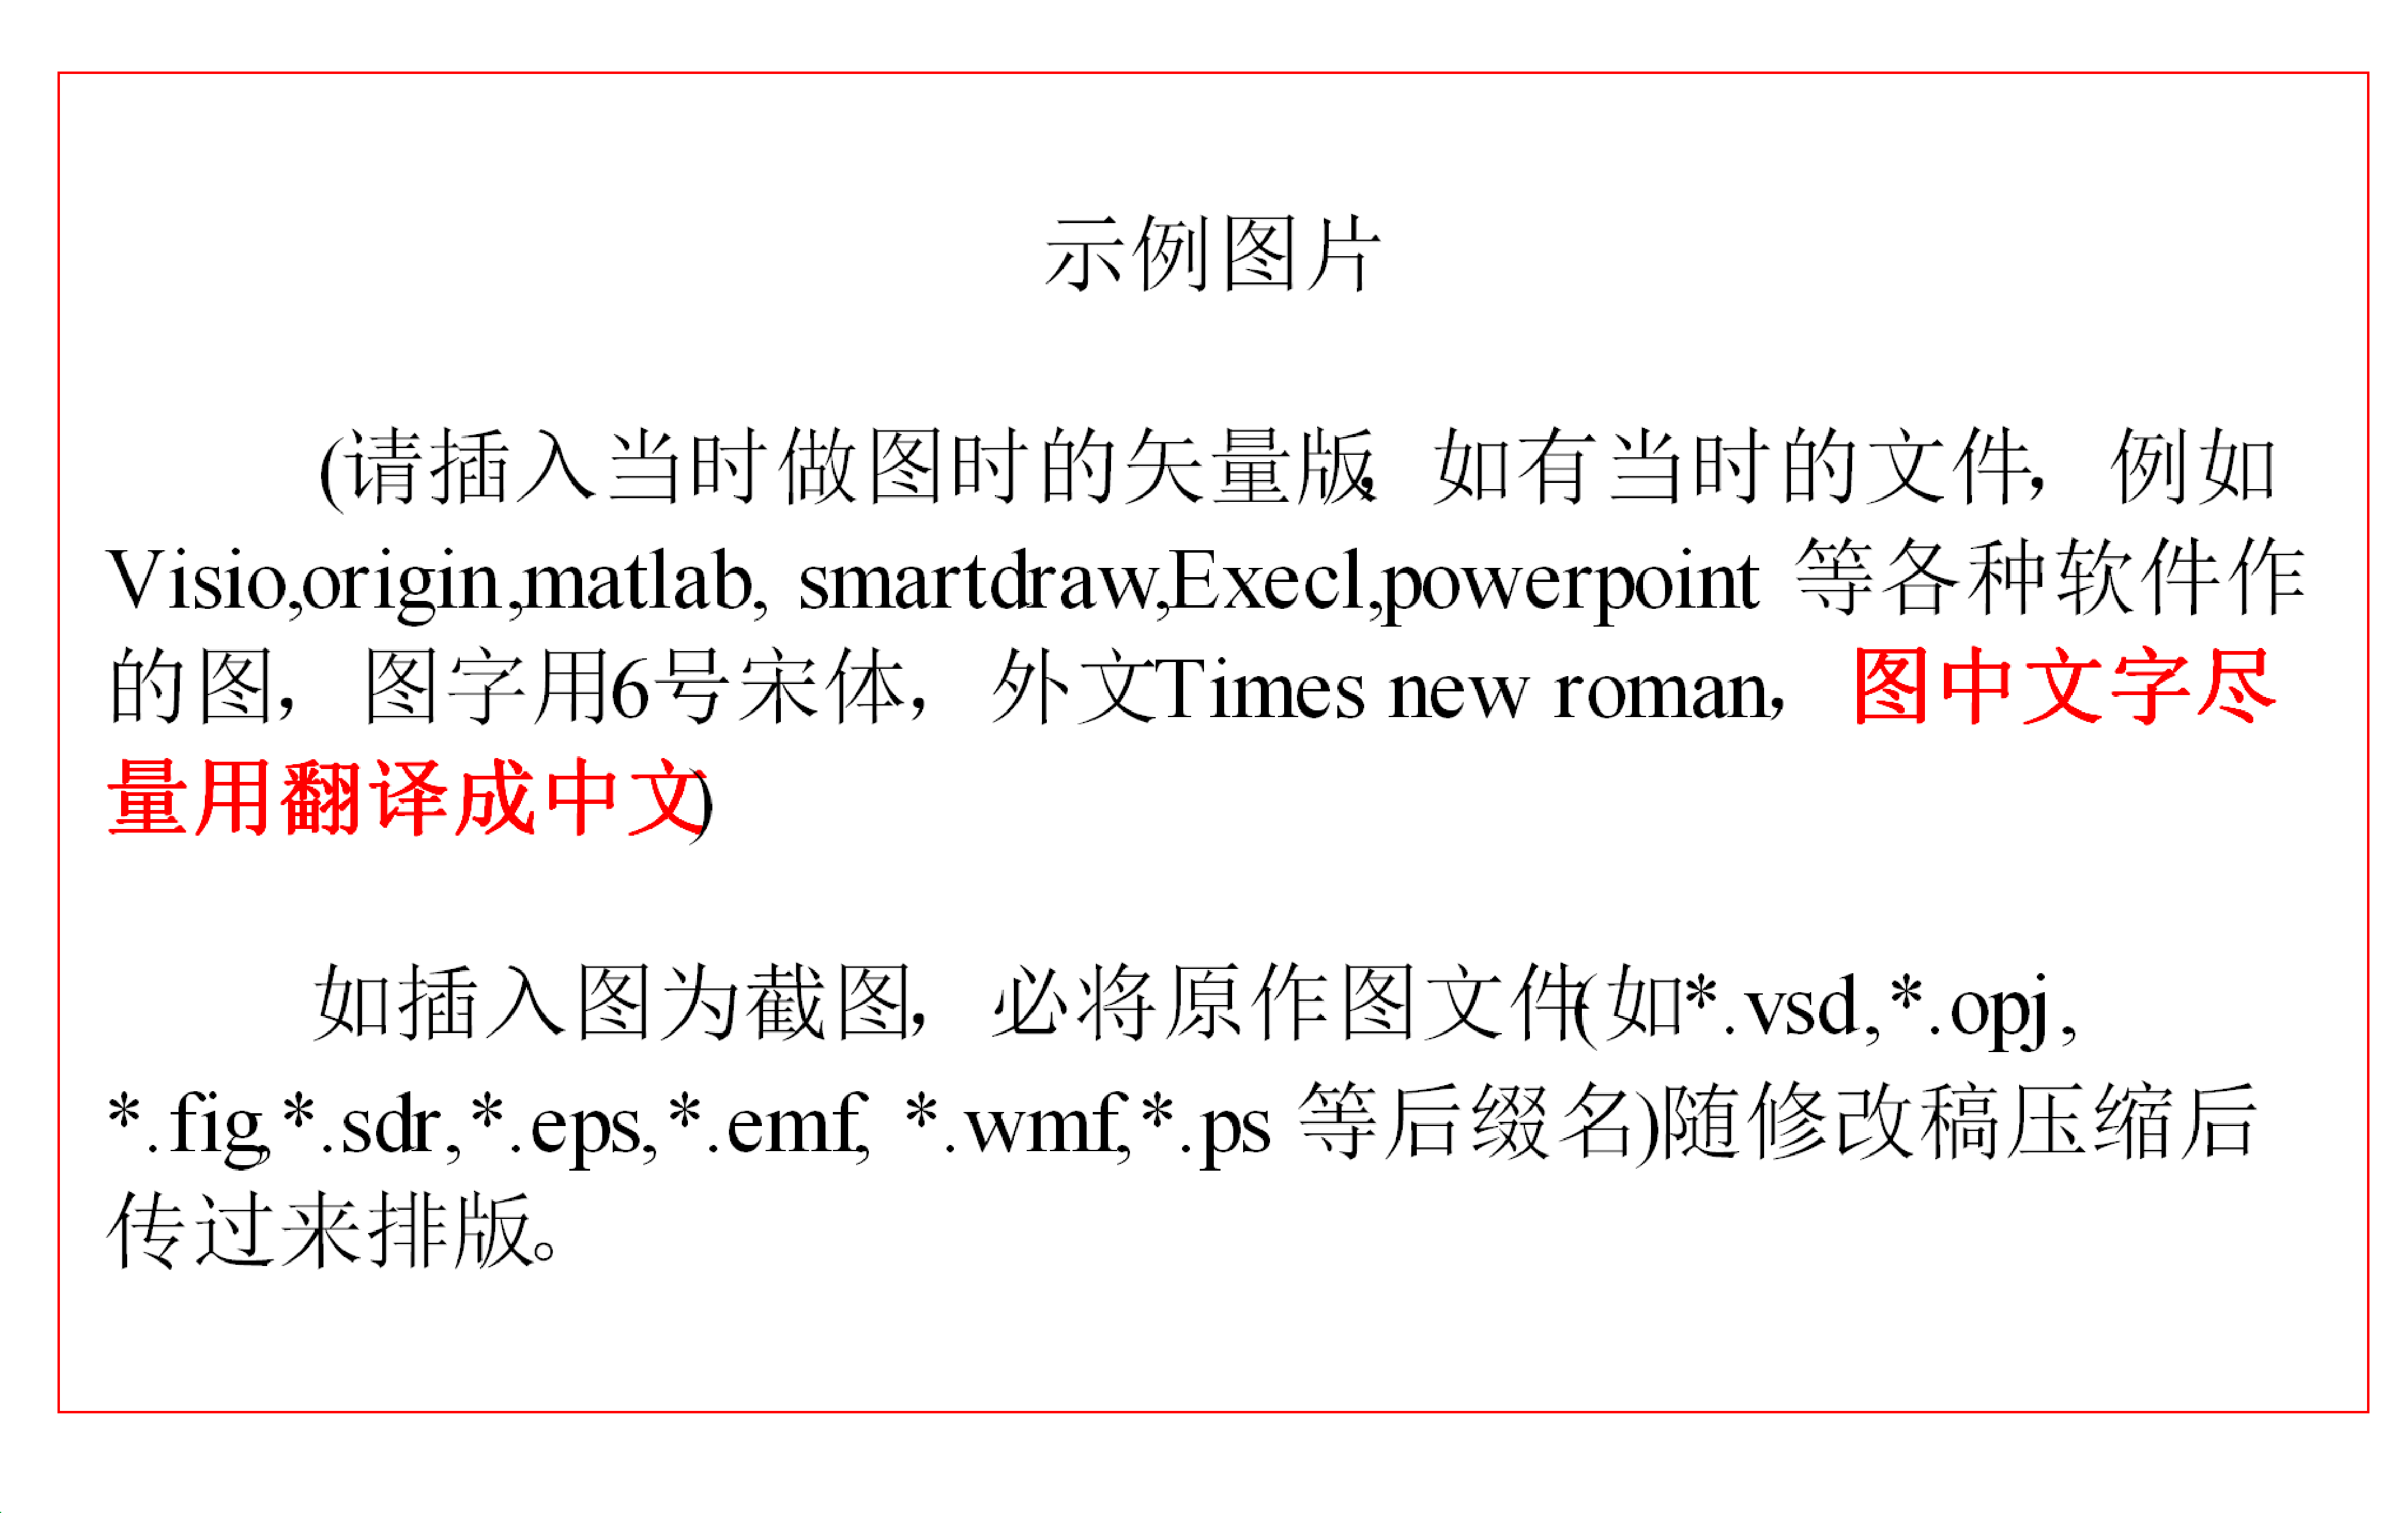
\includegraphics[width=3.15in,height=1.98in]{CJC1.pdf}
  }
  \caption{图片说明}
  \label{fig1}
\end{figure}

\begin{table}[htbp]
  \caption{
    \begin{CJK*}{UTF8}{hei}
      表说明
    \end{CJK*}
  }
  \vspace {-2.5mm}
  \begin{center}
    \begin{tabular}{ll}
      \toprule
      *示例表格*&*第1行为表头,表头要有内容* \\
      \hline
      &
      \\
      &
      \\
      &
      \\
      &
      \\
      \bottomrule
    \end{tabular}
    \label{tab1}
  \end{center}
\end{table}


% 致谢
\vspace{3mm}
\zihao{5}{
  \noindent
  \begin{CJK*}{UTF8}{hei}
    致\quad 谢
  \end{CJK*}\quad 
  \begin{CJK*}{UTF8}{kai} 
    路漫漫其修远兮,吾将上下而求索。
  \end{CJK*}
}

% 参考文献
\vspace{5mm}
\centerline{
  \begin{CJK*}{UTF8}{hei}\zihao{5}
    参~考~文~献
  \end{CJK*}
}
% 使用 BibTeX,请编辑 ref.bib 文件
\bibliographystyle{abbrv}
\zihao{5-} \addtolength{\itemsep}{-1em}
\vspace {1.5mm}
\bibliography{ref}

% \begin{biography}[yourphotofilename.jpg]
% \noindent
% \textbf{First A. Author}\ \ *计算机学报第1作者提供照片电子图片,尺寸为1寸。英文作者介绍内容包括:出生年,学位(或目前学历),职称,主要研究领域(\textbf{与中文作者介绍中的研究方向一致}).*
% *字体为小5号Times New Roman*

% \end{biography}

% \zihao{5-}{
% \setlength\parindent{2em}
% *论文背景介绍为\textbf{英文},字体为小5号Times New Roman体*

% 论文后面为400单词左右的英文背景介绍。介绍的内容包括:

% 本文研究的问题属于哪一个领域的什么问题。该类问题目前国际上解决到什么程度。

% 本文将问题解决到什么程度。

% 课题所属的项目。

% 项目的意义。

% 本研究群体以往在这个方向上的研究成果。

% 本文的成果是解决大课题中的哪一部分,如果涉及863$\backslash
% $973以及其项目、基金、研究计划,注意这些项目的英文名称应书写正确。}

\end{CJK*}
\end{document}


